\section{Experiment Design}
\subsection{Research Questions}
 To systematically investigate whether tuning can improve the 
 performance of baseline methods compared with deep learning method, we set
 the following three research questions:
 
 \bi
 \item RQ1: Can we reproduce Xu et al.'s baseline results (wordembedding+SVM)?
 \item RQ2: Is tuning SVM comparable with Xu et al.'s deep learning method in terms of performance scores?
 \item RQ3: Is tuning SVM comparable with Xu et al.'s deep learning method in terms of runtime?
 \ei
 
 RQ1 is to investigate whether our implementation of wordbedding +SVM method has
 the similar performance with Xu et al.'s baseline, which makes sure that our following 
 analysis can be generalized to Xu et al.'s conclusion. RQ2 and RQ3 lead us to
 investigate whether tuning SVM comparable with Xu et al.'s deep learning from both 
 performance and cost aspects.
 
 \begin{figure}
    \centering
    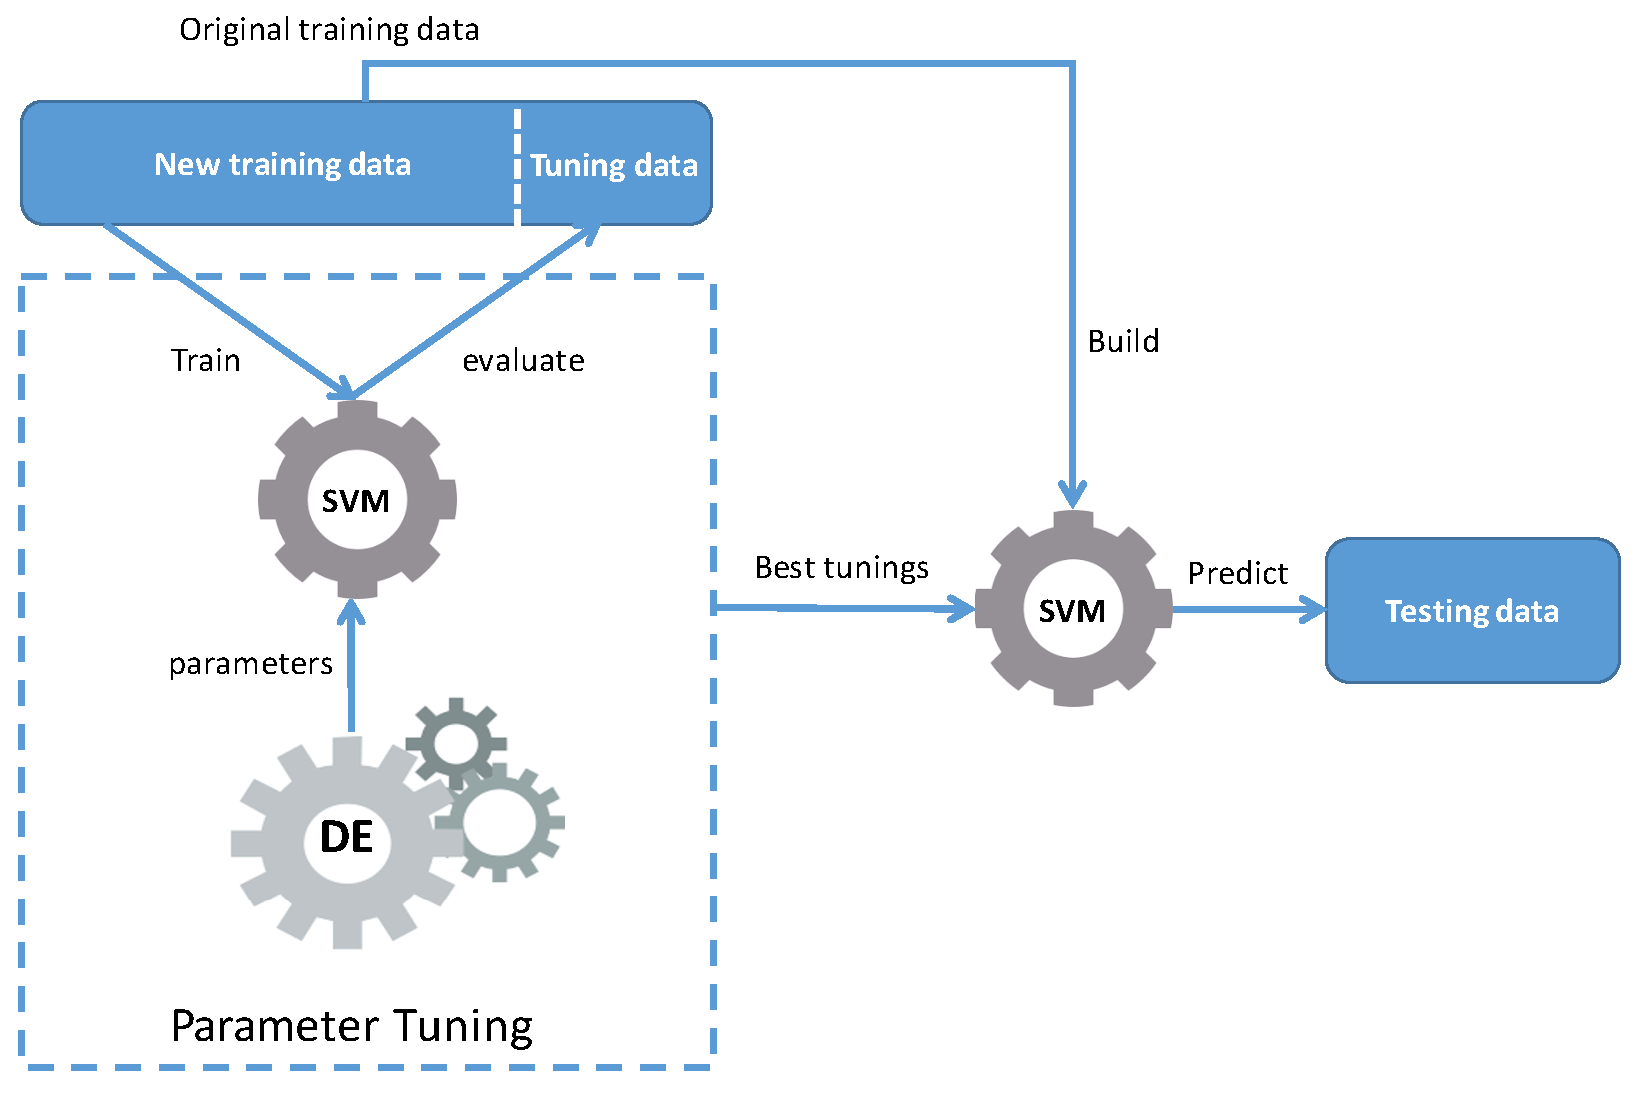
\includegraphics[width=0.5\textwidth]{pic/workflow.pdf}
    \caption{The Overall Workflow of SVM with Parameter Tuning.}
    \label{fig:workflow}
\end{figure}

\subsection{Dataset}
Our experimental data comes from Stack Overflow data dump of 
September 2016\footnote{https://archive.org/details/stackexchange},
where {\it posts} table includes all the questions and answers posted on Stack Overflow
up to date and the {\it postlinks} table describes the relationships between posts, 
e.g., {\it duplicate} and {\it linked}. As mentioned in Section
\ref{problem}, we have four different types of relationships in knowledge units.
Therefore,  {\it linked} type is further divided into {\it indirectly linked} and {\it directly linked}.
Overall, four different types of data are generated according the following rules:
\bi
\item Randomly select a pair of posts from the {\it postlinks} table, if the value
in  {\it PostLinkTypeId} field for this pair of posts is $3$, then this pair of posts is {\it duplicate} posts. 
Otherwise they're {\it directly linked} posts.

\item Randomly select a pair of posts from the {\it posts} table, if this pair of posts is linkable from each other according to
{\it postlinks} table and the distance between them are greater than 2, then this pair of posts is indirectly linked. If they're
not linkable, then this pair of posts is {isolated}.
\ei

In this work, we use the same training and testing
knowledge pairs as in~\cite{xu2016predicting}\footnote{https://github.com/XBWer/ASEDataset}, 
where 6,400 pairs of  knowledge units for training and 1,600 pairs for testing. And each type 
of linked knowledge units accounts for $1/4$ in both training and testing data. The reasons are:
\bi
\item It's to insure that  performance of our baseline method are as closed to Xu et al.'s as possible.
\item Since deep learning method is way complicate compared with SVM and a little difference in implementations
might lead to different results, to fairly compare with Xu et al's result, we simply use the  performance scores
of CNN method from~\cite{xu2016predicting} without any implementation bias introduced.
\ei

For training word2vec model, we randomly select 100,000 knowledge
 units(title, question body and all the answers) from {\it posts} table that are
 related to ``java''. After that, all the training/tuning/testing knowledge units
 used in this paper are converted into word embedding representations by looking up
 each word in wrod2vec model.
 
As seen in \fig{workflow}, instead of using all the 6,400 knowledge units as training data, 
we split the original training data into {\it new training data} and {\it tuning data}, which are
used during parameter tuning procedure for training SVM and evaluating candidate
parameters offered by DE. Afterwards, the {\it new training} data is again fitted into the SVM
with the optimal parameters found by DE and finally  the performance of the tuned
SVM will be evaluated on the  {\it testing data}.

 To reduce the potential variance caused
by how the original training data is divided, {\it 10-fold cross-validation} is performed, where
each time one fold with $640$ knowledge units paris as the tuning data, and the remaining folds with $5760$
knowledge units as  the new training data, then the output SVM model will be evaluated on the testing data. Therefore,
all the performance scores reported below are averaged values over 10 runs.



\subsection{Evaluation Metrics}
When evaluating the performance of tuning SVM on the
multi-class linkable knowledge units prediction problem,
consistent with Xu et al.\cite{xu2016predicting}, we use accuracy, precision, recall and F1-score
as the evaluation metics.



\begin{table}[h]
\begin{tabu} to 0.9\textwidth{cc|c|c|c|c|l}
\cline{3-6}
& & \multicolumn{4}{ c| }{Classified as} \\ \cline{3-6}
& & $C_1$ & $C_2$ & $C_3$ & $C_4$ \\ \cline{1-6}
\multicolumn{1}{ |c  }{\multirow{4}{*}{Actual} } &
\multicolumn{1}{ |c|| }{$C_1$} & $c_{11}$ & $c_{12}$  & $c_{13}$ & $c_{14}$  & \\ \cline{2-6}
\multicolumn{1}{ |c  }{}                        &
\multicolumn{1}{ |c|| }{$C_2$} & $c_{21}$& $c_{22}$ & $c_{23}$ & $c_{24}$ &  \\ \cline{2-6}
\multicolumn{1}{ |c  }{}                        &
\multicolumn{1}{ |c|| }{$C_3$} & $c_{31}$ & $c_{32}$ & $c_{33}$ & $c_{34}$ & \\ \cline{2-6}
\multicolumn{1}{ |c  }{}                        &
\multicolumn{1}{ |c|| }{$C_4$} & $c_{41}$ & $c_{42}$ & $c_{43}$ & $c_{44}$ & \\ \cline{1-6}
\end{tabu}

\caption {Confusion Matrix.}
\label{tab:confusion}
\end{table}

Given a multi-classification problem with true label $C_1$, 
$C_2$, $C_3$ and $C_4$, we can generate a confusion matrix like \tab{confusion}, 
where the value of $c_{ii}$ represents the number of instances that are correctly classified
by the learner for class $C_i$.


Recall from Algorithm~1 that we call differential evolution once for each
 optimization goal. This section lists those optimization goals.
Let $\{A,B,C,D\}$ denote the
true negatives, 
false negatives, 
false positives, and 
true positives
(respectively) found by a binary detector. 
Certain standard measures can be computed from
$A,B,C,D$, as shown below. Note that for $pf$, the {\em better} scores are {\em smaller}
while
for all other scores, the {\em better} scores are {\em larger}.

{\scriptsize\[
\begin{array}{ll}
pd=recall=&D/(B+D)\\
pf=&C/(A+C)\\ 
prec=precision=&D/(D+C) \\
F =&2*pd*prec/(pd + prec)
\end{array}
\]}

The rest of this paper explores tuning for {\em prec} and {\em F}. As discussed
in \tion{goals}, our point is not that these are best or most important optimization goals.
Indeed, the list of ``most important'' goals is domain-specific (see \tion{goals})
and we only explore these two to illustrate how conclusions can change dramatically
when moving from one goal to another.




\subsection{RQ1}
\subsection{RQ2}
